\documentclass{beamer}

\usepackage{multicol}

\usetheme[subsectionpage=progressbar]{metropolis}
\setbeamertemplate{section in toc}[sections numbered]
\setbeamertemplate{subsection in toc}[subsections numbered]

\setbeamertemplate{frame numbering}[fraction]
% \useoutertheme{miniframes}
% \useinnertheme{rounded}
% \usefonttheme{metropolis}
\usecolortheme{spruce}
% \setbeamercolor{background canvas}{bg=white}
% \usecolortheme{wolverine}

\makeatletter
\setbeamertemplate{section page}{
  \centering
  \begin{minipage}{22em}
    \raggedright
    \usebeamercolor[fg]{section title}
    \usebeamerfont{section title}
    \thesection.~\insertsectionhead\\[-1ex]
    \usebeamertemplate*{progress bar in section page}
    \par
    \ifx\insertsubsectionhead\@empty\else%
      \usebeamercolor[fg]{subsection title}%
      \usebeamerfont{subsection title}%
      \thesection.\thesubsection~\insertsubsectionhead
      \fi
  \end{minipage}
  \par
  \vspace{\baselineskip}
}
\makeatother

% \hypersetup{pdfstartview={Fit}} % fits the presentation to the window when first displayed

\titlegraphic{\hfill
\includegraphics[width=.4\textwidth]{img/logo.png}}
\title{Longest Common Subsequences}
\subtitle{Seminar 2}
\author{\large Joris LIMONIER \hfill \textit{\tiny{Supervised by} \scriptsize George KERCHEV}}
% \institute{University of Luxembourg}
\date{May 31, 2021}



\begin{document}
\metroset{block=fill}

\maketitle

\begin{frame}{Table of Contents}
  \tableofcontents
\end{frame}


\section{Introduction}
\subsection{What are LCS ?}
\begin{frame}{What are LCS ?}
  \begin{block}{Notation}
    ``LCS" = Longest Common Subsequence(s)
  \end{block}
  \uncover<2->{
    \textbf{Example 1}
    \begin{center}
      \begin{tabular}{rccccccccccc}
        \uncover<1->{
        $S_1$ : &
                & \only<1-3>{A}\only<4->{\textcolor{magenta}{\textbf A}}
                & \only<1-4>{B}\only<5->{\textcolor{magenta}{\textbf B}}
                & \only<1-5>{A}\only<6->{\textcolor{magenta}{\textbf A}}
                & \only<1-6>{B}\only<7->{\textcolor{magenta}{\textbf B}}
                & B
        }                                                                 \\
        \uncover<3->{
        $S_2$ : &
                & \only<1-3>{A}\only<4->{\textcolor{magenta}{\textbf A}}
                & A
                & \only<1-4>{B}\only<5->{\textcolor{magenta}{\textbf B}}
                & \only<1-5>{A}\only<6->{\textcolor{magenta}{\textbf A}}
                & \only<1-6>{B}\only<7->{\textcolor{magenta}{\textbf B}}}
      \end{tabular}
    \end{center}
    \uncover<8->{
      \(\implies\) The LCS between $S_1$ and $S_2$ is \, \textcolor{magenta}{\textbf{A B A B}}
    }

    \uncover<9->{
      \vspace{.8cm}
      \textit{NB: LCS may not be unique, \,\textcolor{magenta}{A A B B}\, also works.}
    }
  }
\end{frame}

\begin{frame}[t]
  \textbf{Example 2}\\
  What is the LCS of the following sequences ?
  \begin{center}
    \begin{tabular}{rccccccccccc}
      \only<2>{
        $S_3$ :
       & AABBAABAAABABAAABAAABBABAAABAAABAAA \\
       & AAAABBABBBBAAABABBAABBAABBBBBAAAABA \\
       & BBABAAAABABAABBBABABBBBBAAABBBAABBB \\
       & AABAABBABABAABABBBBBBAABBBBBBAAAAAB \\
       & AABAAAAABAABAABAAABBABBBBABBAAAABBB \\
      }                                      \\
      \only<2>{
        $S_4$ :
       & BABBBABAABAABBBABBABBBBBBBABABAAABB \\
       & BBABBABBABBBABBBABBABBABABABBAABABA \\
       & BAABABAAAABABBABABBAAAABABBAABABABB \\
       & BABBBBBBAABAAABBABBBBAAAAABBBBBAAAB \\
       & ABBAAAABBBABABAABBABBBAABABBBABAABA \\
      }
    \end{tabular}
    \only<3>{
      
\includegraphics[width=.9\textwidth]{img/computing_the_lcs.jpg}
    }
  \end{center}
\end{frame}

\subsection{Why are we interested in LCS ?}


\begin{frame}[t]{Applications}
  \begin{itemize}
    \uncover<2->{\item Bioinformatics: Compare sequences of nucleotides (DNA)}
          \uncover<3->{\item Natural Language Processing: Compare texts}
          \uncover<4->{\item Computer Science: Detect differences in texts}
  \end{itemize}
  \vfill
  \begin{center}
    \only<2>{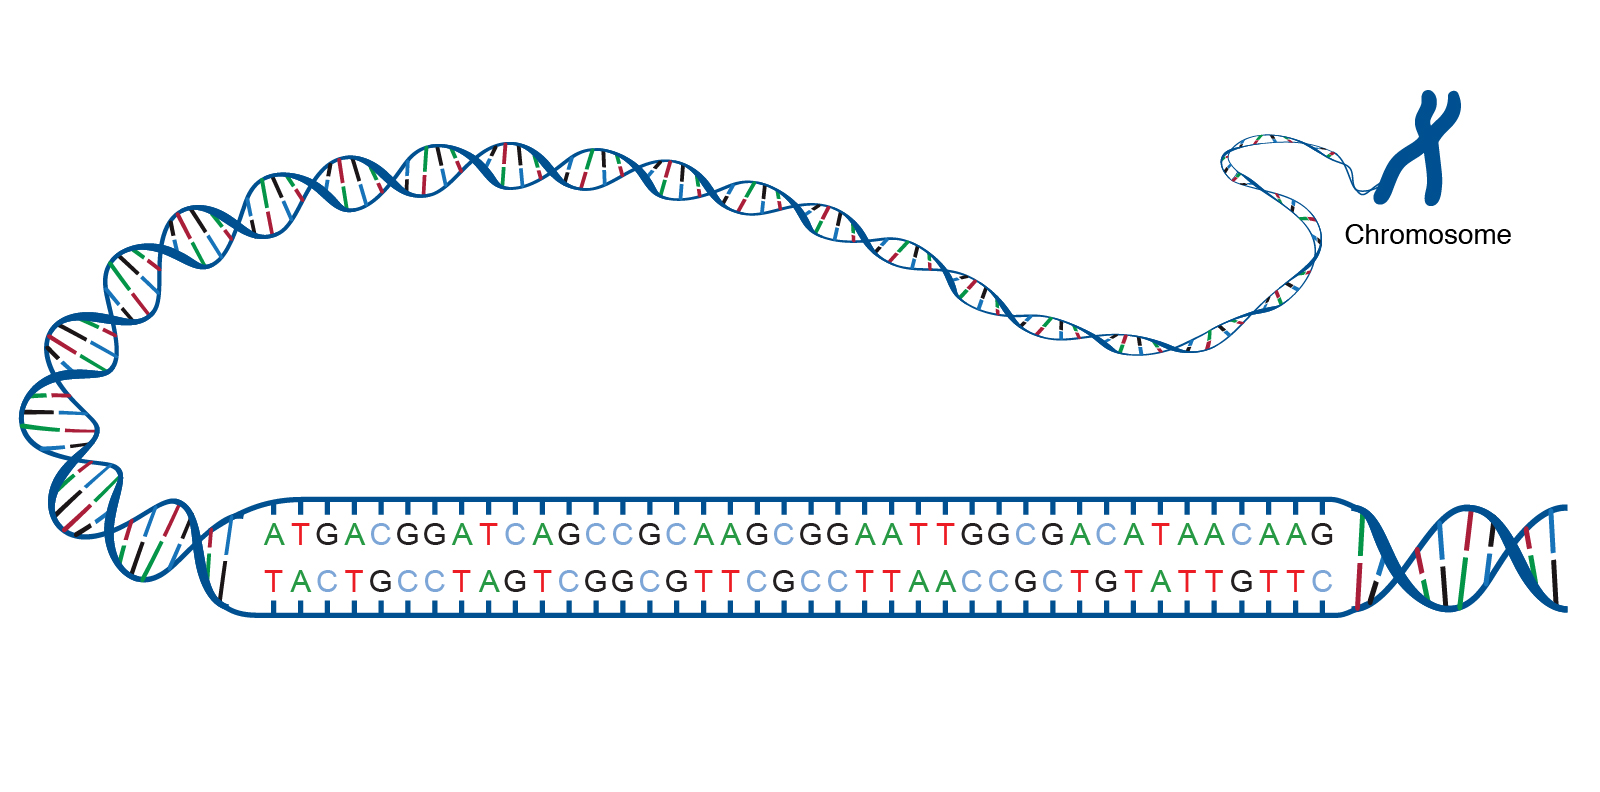
\includegraphics[width=.85\textwidth]{img/dna.jpg}}
    \only<3>{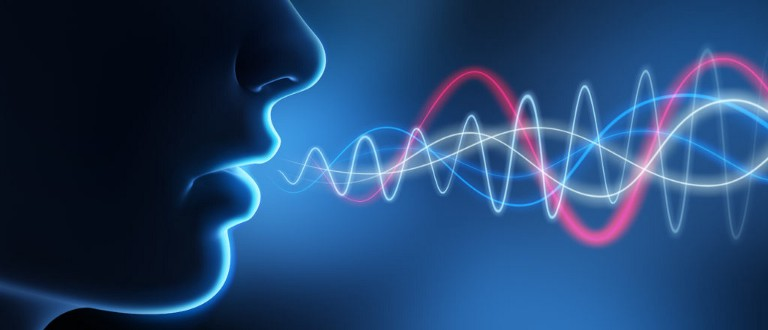
\includegraphics[width=1\textwidth]{img/nlp.jpeg}}
    \onslide<4>{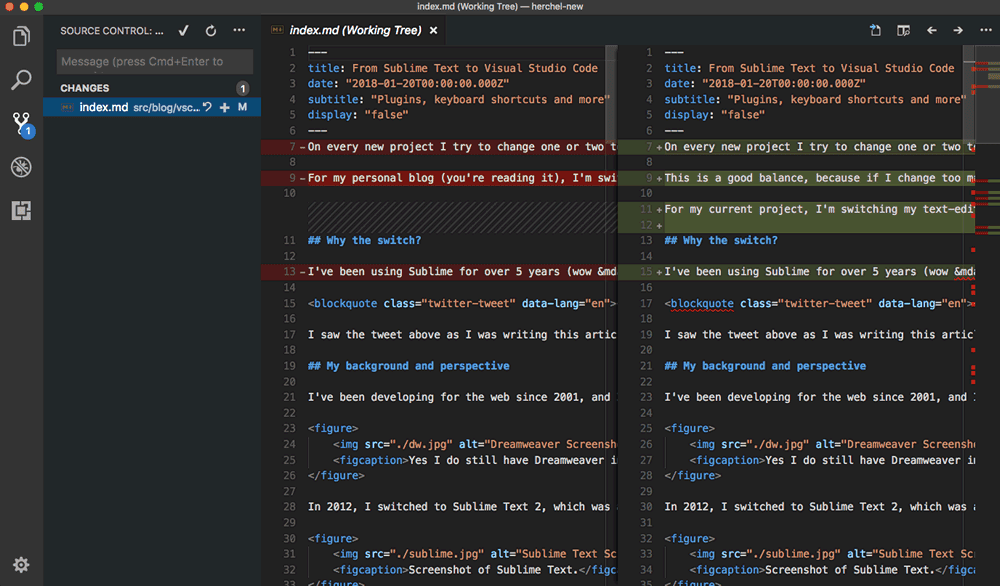
\includegraphics[width=.9\textwidth]{img/file_comparison.png}}
  \end{center}
\end{frame}

\section{How to find LCS ?}
\subsection{Step A: Building the table}

\begin{frame}{Set-up}
  Let \(S_1 = ABABB\) and \(S_2 = AABAB\). \\
  \begin{itemize}
    \uncover<2->{\item Make a table where \(S_1\) and \(S_2\) are the column and row names respectively.}
          \uncover<3->{\item Add a row (resp. column) at the top (resp. left) of the table. Fill them with 0's.}
  \end{itemize}
  \uncover<2->{
    \vfill
    \begin{center}
      \vfill
      \begin{tabular}{|c|c|c|c|c|c|c|}
        \hline
        \only<3->{               & $\varnothing$} & A & B & A & B & B \\
        \hline
        \only<3->{$\varnothing$  & 0              & 0 & 0 & 0 & 0 & 0 \\
          \hline}
        A             \only<3->{ & 0}             &   &   &   &   &   \\
        \hline
        A             \only<3->{ & 0}             &   &   &   &   &   \\
        \hline
        B             \only<3->{ & 0}             &   &   &   &   &   \\
        \hline
        A             \only<3->{ & 0}             &   &   &   &   &   \\
        \hline
        B             \only<3->{ & 0}             &   &   &   &   &   \\
        \hline
      \end{tabular} \\
    \end{center}
  }
\end{frame}

\begin{frame}{Procedure}
  \uncover<1->{
    Start from top-left corner. Move left to right, line by line.
    \begin{itemize}
      \item If row and column names match, increment adjascent top-left-diagonal cell by 1.
      \item Else take the maximum of top and left cells.
    \end{itemize}
  }
  \uncover<1->{
    \begin{center}
      \begin{tabular}{|c|c|c|c|c|c|c|}
        \hline
                      & $\varnothing$ & A             & B             & A             & B             & B             \\
        \hline
        $\varnothing$ & 0             & 0             & 0             & 0             & 0             & 0             \\
        \hline
        A             & 0             & \only{1}<2->  & \only{1}<3->  & \only{1}<4->  & \only{1}<5->  & \only{1}<6->  \\
        \hline
        A             & 0             & \only{1}<7->  & \only{1}<8->  & \only{2}<9-> & \only{2}<10-> & \only{2}<10-> \\
        \hline
        B             & 0             & \only{1}<11-> & \only{2}<11-> & \only{2}<11-> & \only{3}<11-> & \only{3}<11-> \\
        \hline
        A             & 0             & \only{1}<12-> & \only{2}<12-> & \only{3}<12-> & \only{3}<12-> & \only{3}<12-> \\
        \hline
        B             & 0             & \only{1}<13-> & \only{2}<13-> & \only{3}<13-> & \only{4}<13-> & \only{4}<13-> \\
        \hline
      \end{tabular} \\
    \end{center}
  }
\end{frame}

\begin{frame}[standout]
  \(\implies\)\ The length of the LCS is 4.
\end{frame}

\subsection{Step B: Crawling back up the table}
\begin{frame}[t]{Procedure}
  From the table, deduce LCS by starting from the bottom-right cell. Compare cell value with values of top and left cells.
  \begin{itemize}
    \item If cell value \( \in\) \{top cell value, left cell value\}, move to the one with maximum value. \\
    \item Else, add character to LCS and move 1 cell diagonally top-left.
  \end{itemize}
  \uncover<1->{
    \begin{multicols}{2}
      \begin{tabular}{|c|c|c|c|c|c|c|}
        \hline
                                                                &
        $\varnothing$                                           &
        A                                                       &
        B                                                       &
        A                                                       &
        B                                                       &
        B
        \\
        \hline
        $\varnothing$                                           &
        \only{0}<-8> \only{\textcolor{pink}{\textbf 0}}<9->    &
        0                                                       &
        0                                                       &
        0                                                       &
        0                                                       &
        0
        \\
        \hline
        A                                                       &
        0                                                       &
        \only{1}<-7>\only{\textcolor{magenta}{\textbf 1}}<8->     &
        1                                                       &
        1                                                       &
        1                                                       &
        1
        \\
        \hline
        A                                                       &
        0                                                       &
        \only{1}<-6> \only{\textcolor{pink}{\textbf 1}}<7-> &
        1                                                       &
        2                                                       &
        2                                                       &
        2
        \\
        \hline
        B                                                       &
        0                                                       &
        1                                                       &
        \only{2}<-5> \only{\textcolor{magenta}{\textbf 2}}<6-> &
        2                                                       &
        3                                                       &
        3
        \\
        \hline
        A                                                       &
        0                                                       &
        1                                                       &
        2                                                       &
        \only{3}<-4> \only{\textcolor{magenta}{\textbf 3}}<5-> &
        3                                                       &
        3
        \\

        \hline
        B                                                       &
        0                                                       &
        1                                                       &
        2                                                       &
        3                                                       &
        \only{4}<-3> \only{\textcolor{magenta}{\textbf 4}}<4-> &
        \only{4}<-2> \only{\textcolor{pink}{\textbf 4}}<3->
        \\
        \hline
      \end{tabular}
      \begin{tabular}{rccccccccccc}
        \uncover<2->{
         &                                                           &  &  &  & \\
         &                                                           &  &  &  & \\
         &                                                           &  &  &  & \\
          LCS :
         & \only<1-6>{\_\_}\only<7->{\textcolor{magenta}{\textbf A}}
         & \only<1-5>{\_\_}\only<6->{\textcolor{magenta}{\textbf B}}
         & \only<1-4>{\_\_}\only<5->{\textcolor{magenta}{\textbf A}}
         & \only<1-3>{\_\_}\only<4->{\textcolor{magenta}{\textbf B}}
        }                                                                       \\
      \end{tabular}
    \end{multicols}
  }
\end{frame}

\section{Data analysis of LCS results}
\subsection{Average LCS length}
\subsection{Normal fit}

\begin{frame}

\end{frame}

\begin{frame}[standout]
  Thank you
\end{frame}

\end{document}